\chapter{Problem Search Test}
\label{chap:problem_search_test}
\begin{figure}[b]
	\centering
		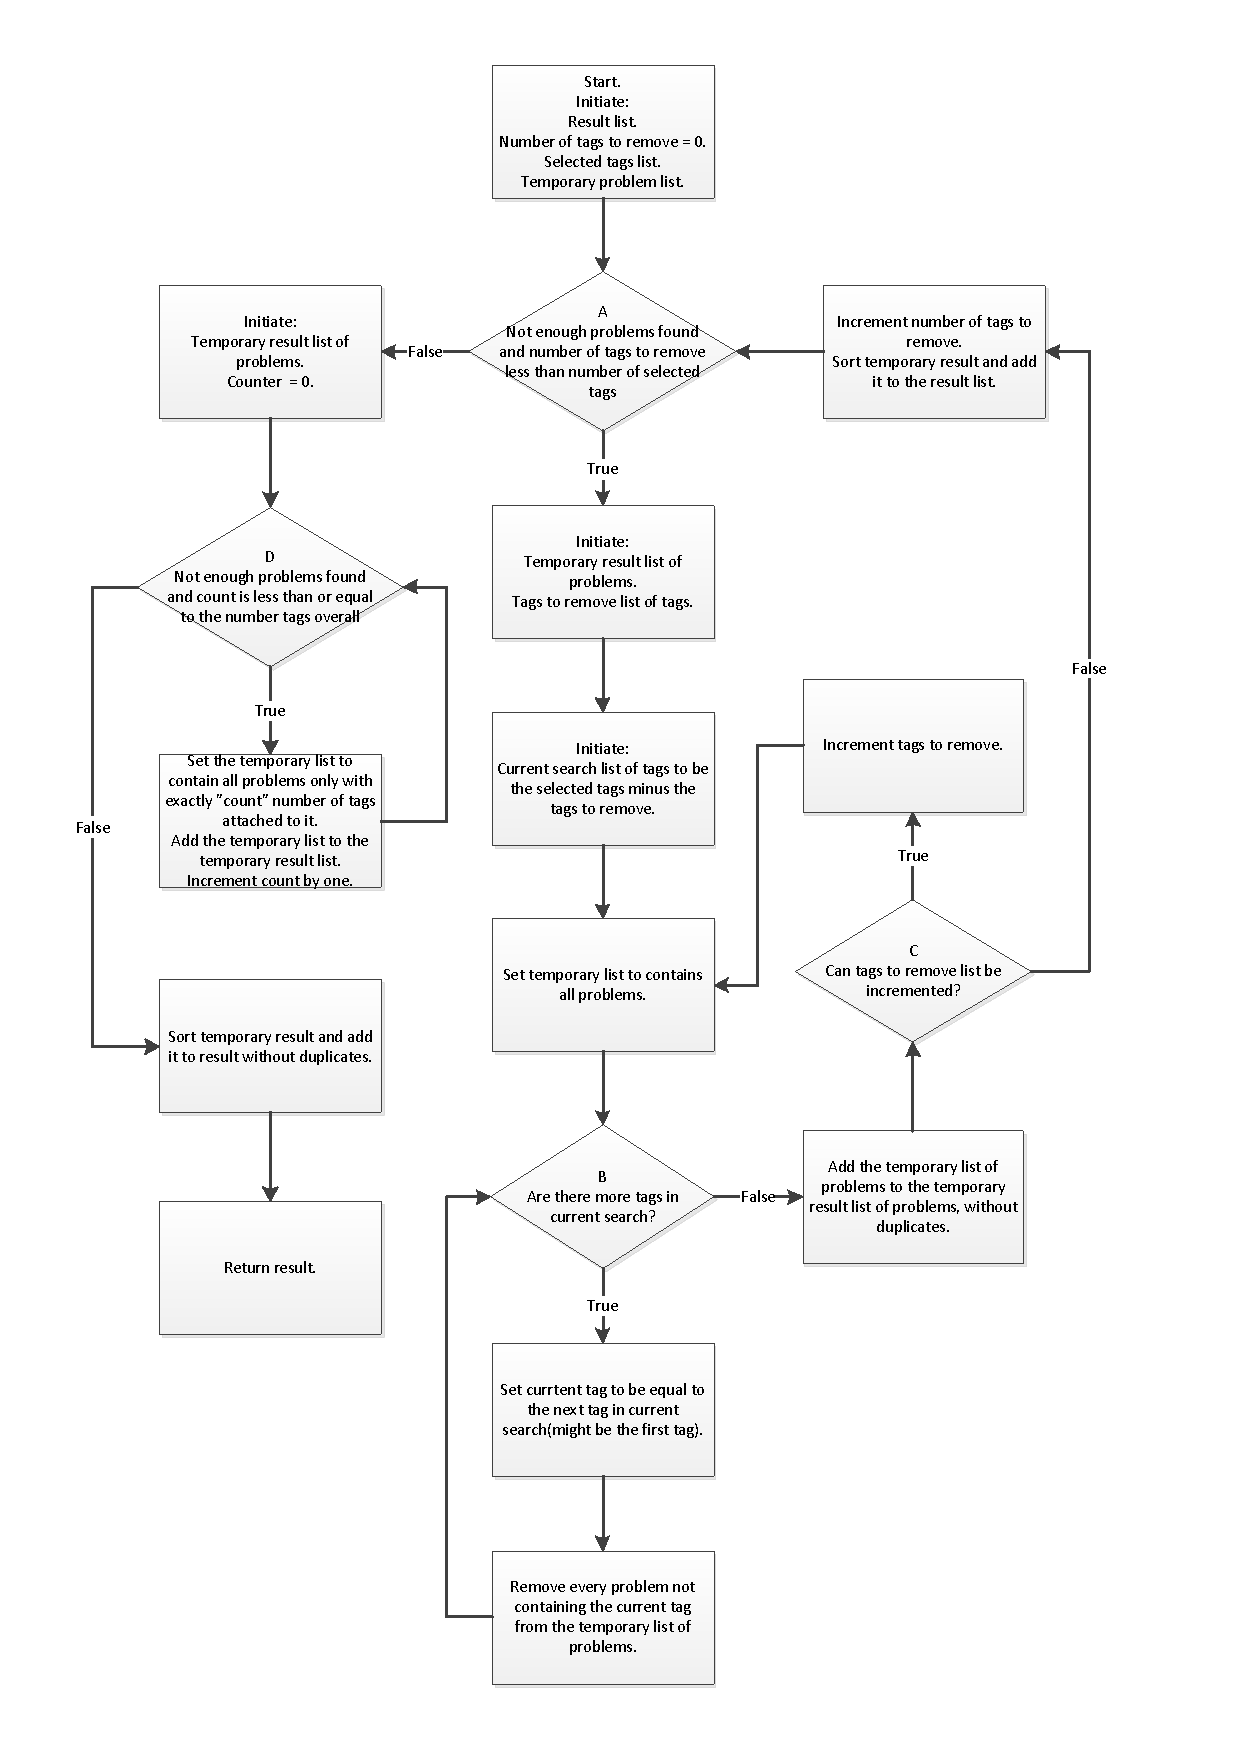
\includegraphics[width=1.00\textwidth]{input/testing/problem_search.pdf}
	\morscaption{Flow chart of the search function.
	The letters in the decisions indicates which loop they are associated with, e.g. the decision labeled A is associated with the loop A}
	\label{fig:problem_search}
\end{figure}

To test our problem search function, we have made an analysis of the code paths of the function.
The flow chart generated from this analysis is seen in figure \ref{fig:problem_search}.
The decisions in the figure are labeled with a letter.
This is done because we want to refer to these decisions -- which are the conditions for loops to run another iteration -- later.
Notice that the loop labeled C is portrayed as a do-while even though code snippet \ref{src:search} shows that this loop is a while loop.
The reason for this is that the loop is a \verb|while(true)|, which breaks when an exception of the type \cl{NotSupportedException} is thrown.
This means that the loop will always run at least once, like a do-while loop.
This is more thoroughly described in subsection \ref{sub:searchTags}.

Since the search method only contain loops and no if statements, the focus for the test cases regarding the search is on the loops edge conditions.
The first test case will consider the option where the none of the loop is not run.
If A is not run, B and C will never be run because they are inside of the A loop.
A will not be run if either the size of the result is at least equal to the minimum number of problems to find or if the number of tags to remove is at least equal to the number of selected tags.
To not run the A loop, the number of selected tags is set to 0, i.e. no tags are selected.
In order for D loop not to run there has been found enough problems or if the \vari{count} variable is at least equal